% Diagrama D — os três níveis analíticos do perfil de cooperação preditiva
% e sua complementaridade: (a) correlação de ranking; (b) matriz de
% vencedores W com propagação de empate; (c) matriz de inversões R.
\documentclass[tikz,border=6pt]{standalone}
% Preâmbulo compartilhado dos diagramas conceituais do relatório CoInfoSim.
% Compilação: xelatex (determinística; nenhum dado experimental é usado).
\usepackage{fontspec}
\setmainfont{Liberation Sans}
\setsansfont{Liberation Sans}
\usepackage{amsmath}
\usepackage{bm}
\usepackage{tikz}
\usetikzlibrary{arrows.meta,positioning,calc,fit,backgrounds,decorations.pathreplacing,matrix,patterns}
\definecolor{CoinAccent}{RGB}{25,80,140}
\definecolor{CoinAccentDark}{RGB}{18,55,95}
\definecolor{CoinAccentPale}{RGB}{237,242,248}
\definecolor{CoinGray}{RGB}{95,95,95}
\definecolor{CoinGrayPale}{RGB}{246,246,246}
\definecolor{CoinWin}{RGB}{76,140,90}    % verde discreto (vitória)
\definecolor{CoinLose}{RGB}{182,88,79}   % vermelho discreto (derrota)
\tikzset{
  bloco/.style={draw=CoinAccentDark, fill=CoinAccentPale, rounded corners=1.2pt,
                align=center, font=\small, inner sep=4pt, minimum height=7mm},
  bloconeutro/.style={draw=CoinGray, fill=CoinGrayPale, rounded corners=1.2pt,
                align=center, font=\small, inner sep=4pt, minimum height=7mm},
  blocoreal/.style={draw=CoinAccentDark, fill=white, rounded corners=1.2pt,
                align=center, font=\small, inner sep=4pt, minimum height=7mm},
  seta/.style={-{Stealth[length=2.4mm]}, thick, CoinAccentDark},
  setacinza/.style={-{Stealth[length=2.4mm]}, thick, CoinGray},
  rotulo/.style={font=\footnotesize\itshape, text=CoinGray, align=center},
}

\begin{document}
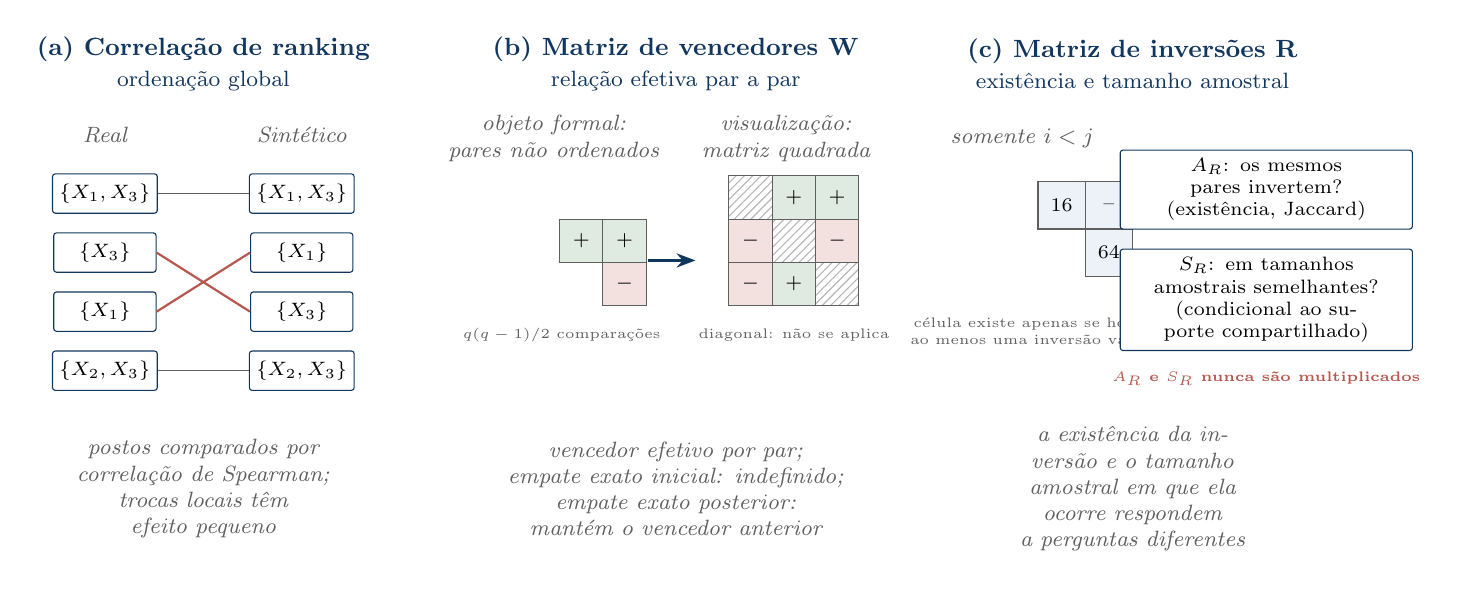
\begin{tikzpicture}
  \tikzset{itemrank/.style={draw=CoinAccentDark, fill=white, rounded corners=1pt,
            font=\scriptsize, inner sep=2.5pt, minimum width=13mm, minimum height=5mm}}

  % ------------------------------------------------------------------ (a)
  \begin{scope}
    \node[font=\small\bfseries, text=CoinAccentDark, align=center] at (1.6,4.9)
      {(a) Correlação de ranking\\ \normalfont\footnotesize ordenação global};
    \node[rotulo] at (0.35,4.0) {Real};
    \node[rotulo] at (2.85,4.0) {Sintético};
    % listas ordenadas por perda (menor no topo); uma troca entre 2º e 3º
    \foreach \i/\lab in {1/{$\{X_1,X_3\}$}, 2/{$\{X_3\}$}, 3/{$\{X_1\}$}, 4/{$\{X_2,X_3\}$}}{
      \node[itemrank] (ra\i) at (0.35,4.0-\i*0.75) {\lab};
    }
    \foreach \i/\lab in {1/{$\{X_1,X_3\}$}, 2/{$\{X_1\}$}, 3/{$\{X_3\}$}, 4/{$\{X_2,X_3\}$}}{
      \node[itemrank] (rb\i) at (2.85,4.0-\i*0.75) {\lab};
    }
    \draw[CoinGray] (ra1.east) -- (rb1.west);
    \draw[CoinLose, thick] (ra2.east) -- (rb3.west);
    \draw[CoinLose, thick] (ra3.east) -- (rb2.west);
    \draw[CoinGray] (ra4.east) -- (rb4.west);
    \node[rotulo, text width=3.7cm] at (1.6,-0.5)
      {postos comparados por\\correlação de Spearman;\\trocas locais têm efeito pequeno};
  \end{scope}

  % ------------------------------------------------------------------ (b)
  \begin{scope}[xshift=5.1cm]
    \node[font=\small\bfseries, text=CoinAccentDark, align=center] at (2.5,4.9)
      {(b) Matriz de vencedores $\mathbf{W}$\\ \normalfont\footnotesize relação efetiva par a par};
    % objeto formal triangular (3 subconjuntos, 3 pares)
    \node[rotulo] at (0.95,3.95) {objeto formal:\\pares não ordenados};
    \foreach \r/\c/\v/\cor in {1/2/{$+$}/CoinWin, 1/3/{$+$}/CoinWin, 2/3/{$-$}/CoinLose}{
      \node[draw=CoinGray, fill=\cor!18, minimum size=5.5mm, font=\scriptsize, inner sep=0pt]
        at ($(0.2,3.2)+(\c*0.55,-\r*0.55)$) {\v};
    }
    \node[rotulo, font=\tiny] at (1.05,1.45) {$q(q-1)/2$ comparações};
    \draw[seta] (2.15,2.4) -- (2.75,2.4);
    % visualização quadrada redundante
    \node[rotulo] at (3.9,3.95) {visualização:\\matriz quadrada};
    \foreach \r/\c/\v/\cor in {1/2/{$+$}/CoinWin, 1/3/{$+$}/CoinWin, 2/3/{$-$}/CoinLose,
                               2/1/{$-$}/CoinLose, 3/1/{$-$}/CoinLose, 3/2/{$+$}/CoinWin}{
      \node[draw=CoinGray, fill=\cor!18, minimum size=5.5mm, font=\scriptsize, inner sep=0pt]
        at ($(2.9,3.75)+(\c*0.55,-\r*0.55)$) {\v};
    }
    \foreach \r in {1,2,3}{
      \node[draw=CoinGray, pattern=north east lines, pattern color=CoinGray!45,
            minimum size=5.5mm, inner sep=0pt]
        at ($(2.9,3.75)+(\r*0.55,-\r*0.55)$) {};
    }
    \node[rotulo, font=\tiny] at (4.0,1.45) {diagonal: não se aplica};
    \node[rotulo, text width=4.6cm] at (2.5,-0.5)
      {vencedor efetivo por par;\\empate exato inicial: indefinido;\\empate exato posterior: mantém o vencedor anterior};
  \end{scope}

  % ------------------------------------------------------------------ (c)
  \begin{scope}[xshift=11.1cm]
    \node[font=\small\bfseries, text=CoinAccentDark, align=center] at (2.3,4.9)
      {(c) Matriz de inversões $\mathbf{R}$\\ \normalfont\footnotesize existência e tamanho amostral};
    % matriz triangular 3x3 esquemática: apenas i<j, valores = último n de inversão
    \node[rotulo] at (0.9,3.95) {somente $i<j$};
    \foreach \r/\c/\v in {1/2/{16}, 1/3/{--}, 2/3/{64}}{
      \node[draw=CoinGray, fill=CoinAccentPale, minimum size=6mm, font=\scriptsize, inner sep=0pt]
        at ($(0.2,3.7)+(\c*0.6,-\r*0.6)$) {\v};
    }
    \node[rotulo, font=\tiny, text width=3.3cm] at (1.05,1.5) {célula existe apenas se houve\\ ao menos uma inversão válida};
    % dois indicadores separados, nunca multiplicados
    \node[draw=CoinAccentDark, rounded corners=1pt, fill=white, font=\scriptsize,
          text width=3.5cm, align=center, inner sep=3pt] (arbox) at (4.0,3.3)
      {$A_R$: os mesmos pares invertem?\\(existência, Jaccard)};
    \node[draw=CoinAccentDark, rounded corners=1pt, fill=white, font=\scriptsize,
          text width=3.5cm, align=center, inner sep=3pt] (srbox) at (4.0,1.9)
      {$S_R$: em tamanhos amostrais semelhantes?\\(condicional ao suporte compartilhado)};
    \node[rotulo, font=\tiny\bfseries, text=CoinLose] at (4.0,0.9) {$A_R$ e $S_R$ nunca são multiplicados};
    \node[rotulo, text width=4.6cm] at (2.3,-0.5)
      {a existência da inversão e o tamanho\\amostral em que ela ocorre respondem\\a perguntas diferentes};
  \end{scope}
\end{tikzpicture}
\end{document}
